At this point, we turn on the interaction. We study interacting bosons in an elliptical harmonic trap. We use the values of $\xi_1$ and $\xi_2$ found in the previous section and we proceed to increase the number of particles to be able to benchmark our results to the ones found in \cite{DalfString}.
 
As we increase the number of particles, we note that the computational time increases dramatically as well as the system becomes more unstable. With the learning rate chosen before, the energy diverges immediately. It is clear that we need to chose a much smaller learning rate. Moreover we need to take into account the number of hidden nodes: the results are more truthful as the number of hidden nodes increases until the point in which it does not make any sense to increase them anymore (until $N_p\times $D). Therefore for each configuration (number of particles, number of dimensions) we chose M as the greater one which keeps the stability and we balance this choice by decreasing the learning rate.

\begin{figure}[H]
%	\centering
%	\begin{subfigure}[b]{1.0\textwidth}
%		\centering
%		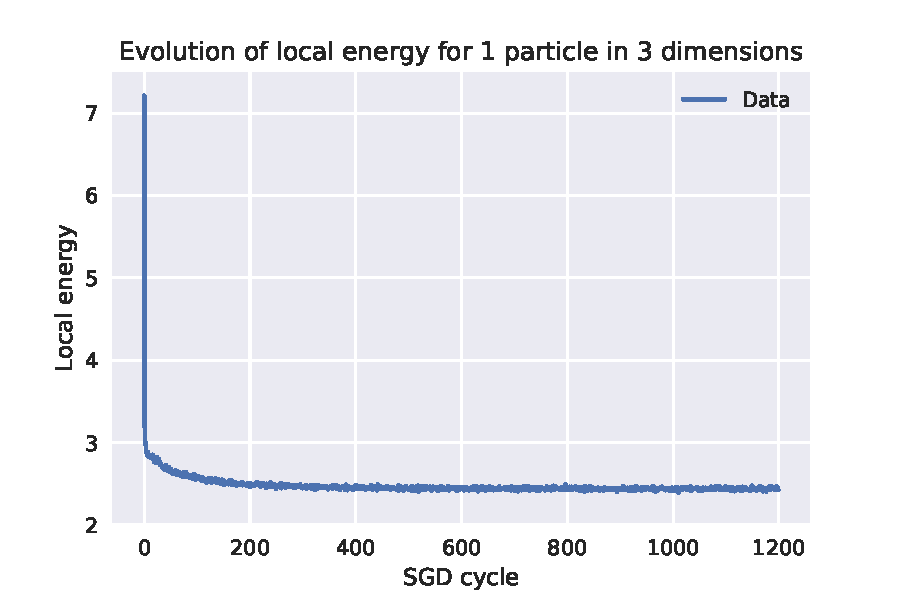
\includegraphics[width=\textwidth]{plot_final1_2.pdf}
%		\caption{}
%	\end{subfigure}
		\centering
		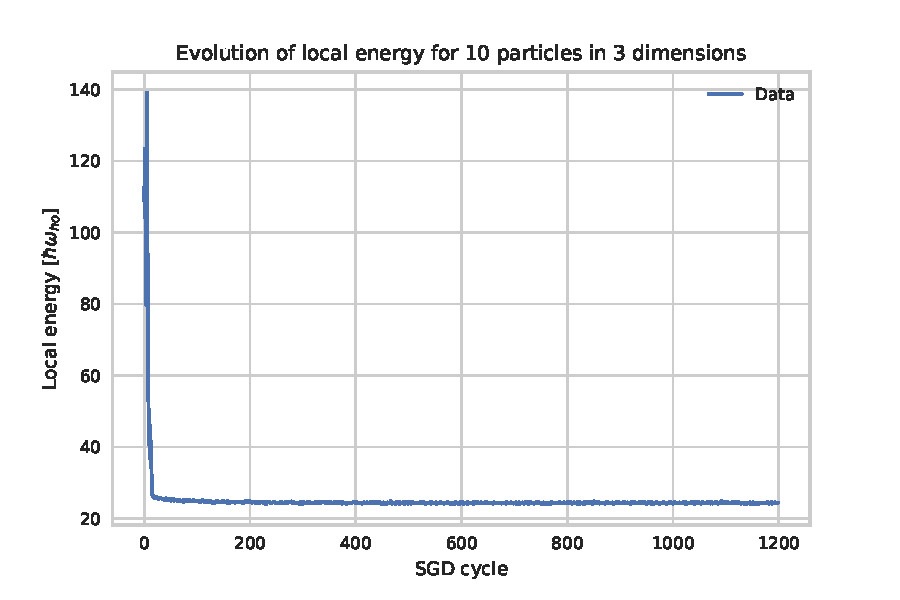
\includegraphics[scale=1.0]{plot_final10.pdf}
	\caption{In this figures, we plot the evolution of ten particles in three dimensions as the program adapts with SGD. We use M $=8$ and $\eta=0.01$. As we can see the local energy converges quickly.}
	\label{Fig:7_8}
\end{figure}

We plot in Fig. (\ref{Fig:7_8}) the results of the first configuration carried out with a $\sigma$ (which gives the spread of the initial parameters according to a Gaussian distribution) of $0.1$ to prove that the RBM is effectively learning. Nevertheless, we note that after $N_p=10$ we need to increase M since the number of particles increases. This process requires to decrease the learning rate to keep stability. By consequence the program becomes much slower to converge to a value: the increment of computational time is dramatic. Therefore, we decide to decrease $\sigma$ to the value of $0.01$. With this choice, we can save some SGD cycle since we have already proven the learning of the RBM. Since we need a much greater number of SGD cycles to find equilibrium with respect to the non-interacting case, we select a number of 1200 SGD cycles. To save time we select $10^5$ MC steps. In the following table we summarize our choices of $N_p$, D, M and we show the results obtained: 


\begin{table}[H]
	\centering
	\caption{Setup used with the various configurations and results obtained: we show the number of hidden nodes $M$, learning rate $\eta$, acceptance rate for each configuration. The learning rate remains constant as we increase the number of particles whereas M is increased each time. The learning rate $\eta$ is the same for $N_p\geq20$. }
	\begin{tabular}{c c |c c c | c} 
		$\boldsymbol{N_p}$ & \textbf{D}  & \textbf{M} & $\boldsymbol{\eta}$ & \textbf{Acceptance rate} &\textbf{Results}\\  
		&&&&&$[\hbar\omega_{ho}]$\\\hline
		10 & 3 & 8 & 0.01  & 0.89 & $\SI{2.44\pm 0.01}{}$ \\
		20 & 3 & 25 & 0.001 & 0.89 & $\SI{2.47\pm 0.01}{}$\\
		30 & 3 & 27 & 0.001 & 0.89 & $\SI{2.47\pm 0.01}{}$\\
		40 & 3 & 30 & 0.001 & 0.89 & $\SI{2.48\pm 0.01}{}$\\
		50 & 3 & 40 & 0.001 & 0.88 & $\SI{2.50 \pm 0.01}{}$\\ 
		60 & 3 & 52 & 0.001 &      &                \\
		70 & 3 & 54 & 0.001 &      &                \\
		80 & 3 & 56 & 0.001 &   0.89   &  $\SI{2.56\pm0.01}{}$              \\
		90 & 3 & 58 & 0.001 &      &                \\
		100 & 3 & 60 &  0.001   &  0.89     &    $\SI{2.63\pm 0.02}{}$           \\
	\end{tabular}
	\label{Tab:4}
\end{table} 

For each configuration, after having checked approximately where the system equilibrates, we take all the mean energies after that point and we take the mean of all of those propagating the uncertainties obtained with the blocking method. The results are shown in Tab. \ref{Tab:4}. 
Furthermore we consider the results obtained from the GP equation in \cite{DalfString} and we check that ours follow the same trend in the small number of particle regime. In Fig. (\ref{Fig:9}), we show how our ML results (blue points) behave in the range $[0,100]$ and $[0,500]$ with respect to GP (red points). The uncertainties are really small, it is not possible to see them from the figure. We plot also the energy per particle with $N_p=1$ (green triangle) which is still a non-interacting case, just as a guide for the reader to follow the GP trend below $N_p=100$. As we can see the energy per particle increases as we increase the number of particles coherently with GP. However, the ML data seem to underestimate the GP trend. This problem could mean that we have not used enough hidden nodes. Nevertheless it should be noted that with $N_p=100$, the maximum number of hidden nodes possible is found to be M $=60$. If we increase M above this value, either the energy diverges immediately or we obtain negative energies. This configuration corresponds to $18360$ variational parameters. This seems to be our limit.\\
The error is quite constant as we increase $N_p$, it grows for $N_p=100$. This is due to the fact that the increment of $N_p$, M makes the system less able to stabilize around a value (the fluctuations become bigger and bigger). In order to decrease the error, we should increase the number of Monte Carlo step, this has not been done here since it would have been computationally too expensive.\\
As regards $E_L/N_p$ for $N_p=100$, in \cite{DalfString} the result of $2.66\ \hbar\omega_{ho}$ is reported. We obtain $\SI{2.63\pm 0.02}{}\ \hbar\omega_{ho}$ which agrees within $2\sigma$ with the GP result. 

\begin{figure}[H]
	\centering
	\centerline{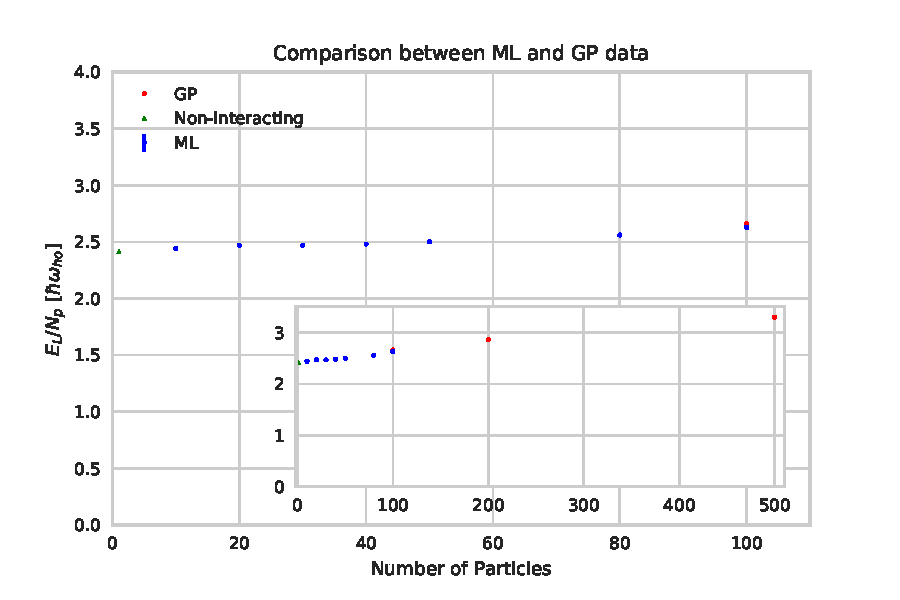
\includegraphics[scale=1.2]{plot_finale.pdf}}
	\caption{Comparison between ML data from our code (blue dots) and the GP results (red dots) in \cite{DalfString} in the range $[0,100]$ and $[0,500]$. The green triangle is the expected $E_L/N_p$ for $N_p=1$: in this situation we are still in the non-interacting case. The point is inserted to help the reader to follow the GP trend below $N_p=100$. ML data seem to underestimate the GP results. This problem is probably related to the insufficient number of hidden nodes used.}
	\label{Fig:9}
\end{figure} 